\documentclass[10pt,landscape]{article}
\usepackage{multicol}
\usepackage{calc}
\usepackage{ifthen}
\usepackage[landscape]{geometry}
\usepackage{graphicx}
\usepackage{amsmath, amssymb, amsthm}
\usepackage{latexsym, marvosym}
\usepackage{pifont}
\usepackage{lscape}
\usepackage{graphicx}
\usepackage{array}
\usepackage{booktabs}
\usepackage[bottom]{footmisc}
\usepackage{tikz}
\usetikzlibrary{shapes}
\usepackage{pdfpages}
\usepackage{xcolor}
\usepackage{wrapfig}
\usepackage{enumitem}
\setlist[description]{leftmargin=0pt}
\usepackage{xfrac}
\usepackage[pdftex,
            pdfauthor={William Chen},
            pdftitle={Probability Cheatsheet},
            pdfsubject={A cheatsheet pdf and reference guide originally made for Stat 110, Harvard's Introduction to Probability course. Formulas and equations for your statistics class.},
            pdfkeywords={probability} {statistics} {cheatsheet} {pdf} {cheat} {sheet} {formulas} {equations}
            ]{hyperref}
\usepackage[
            open,
            openlevel=2
            ]{bookmark}
\usepackage{relsize}
\usepackage{rotating}

 \newcommand\independent{\protect\mathpalette{\protect\independenT}{\perp}}
    \def\independenT#1#2{\mathrel{\setbox0\hbox{$#1#2$}%
    \copy0\kern-\wd0\mkern4mu\box0}} 
    
\newcommand{\noin}{\noindent}    
\newcommand{\logit}{\textrm{logit}} 
% \newcommand{\var}{\textrm{Var}}
\newcommand{\cov}{\textrm{Cov}} 
\newcommand{\corr}{\textrm{Corr}} 
\newcommand{\N}{\mathcal{N}}
\newcommand{\Bern}{\textrm{Bern}}
\newcommand{\Bin}{\textrm{Bin}}
\newcommand{\Beta}{\textrm{Beta}}
\newcommand{\Gam}{\textrm{Gamma}}
\newcommand{\Expo}{\textrm{Expo}}
\newcommand{\Pois}{\textrm{Pois}}
\newcommand{\Unif}{\textrm{Unif}}
\newcommand{\Geom}{\textrm{Geom}}
\newcommand{\NBin}{\textrm{NBin}}
\newcommand{\Hypergeometric}{\textrm{HGeom}}
\newcommand{\HGeom}{\textrm{HGeom}}
\newcommand{\Mult}{\textrm{Mult}}
\newcommand{\mean}{\mathbb{E}}
\newcommand{\var}{\mathbb{V}}
\newcommand{\indicator}{\mathbb{I}}
\newcommand{\inp}{\textbf{x}}
\newcommand{\out}{\textbf{y}}
\newcommand{\parameter}{\boldsymbol{\theta}}
\newcommand{\nlogit}[1]{\log \left( \frac{#1}{1 - #1} \right)}
\newcommand{\R}{\mathbb{R}}


\geometry{top=.4in,left=.2in,right=.2in,bottom=.4in}

\pagestyle{empty}
\makeatletter
\renewcommand{\section}{\@startsection{section}{1}{0mm}%
                                {-1ex plus -.5ex minus -.2ex}%
                                {0.5ex plus .2ex}%x
                                {\normalfont\large\bfseries}}
\renewcommand{\subsection}{\@startsection{subsection}{2}{0mm}%
                                {-1explus -.5ex minus -.2ex}%
                                {0.5ex plus .2ex}%
                                {\normalfont\normalsize\bfseries}}
\renewcommand{\subsubsection}{\@startsection{subsubsection}{3}{0mm}%
                                {-1ex plus -.5ex minus -.2ex}%
                                {1ex plus .2ex}%
                                {\normalfont\small\bfseries}}
\makeatother

\setcounter{secnumdepth}{0}

\setlength{\parindent}{0pt}
\setlength{\parskip}{0pt plus 0.5ex}

% -----------------------------------------------------------------------

\usepackage{titlesec}

\titleformat{\section}
{\color{blue}\normalfont\large\bfseries}
{\color{blue}\thesection}{1em}{}
\titleformat{\subsection}
{\color{cyan}\normalfont\normalsize\bfseries}
{\color{cyan}\thesection}{1em}{}
% Comment out the above 5 lines for black and white

\begin{document}

\raggedright
\footnotesize
\begin{multicols*}{3}

% multicol parameters
% These lengths are set only within the two main columns
%\setlength{\columnseprule}{0.25pt}
\setlength{\premulticols}{1pt}
\setlength{\postmulticols}{1pt}
\setlength{\multicolsep}{1pt}
\setlength{\columnsep}{2pt}

%%%%%%%%%%%%%%%%%%%%%%%%%%%%%%%%%%%%
%%% TITLE
%%%%%%%%%%%%%%%%%%%%%%%%%%%%%%%%%%%%

\begin{center}
    {\color{blue} \Large{\textbf{Probability for ML Cheatsheet}}} \\
   % {\Large{\textbf{Probability Cheatsheet}}} \\
    % comment out line with \color{blue} and uncomment above line for b&w
\end{center}

%%%%%%%%%%%%%%%%%%%%%%%%%%%%%%%%%%%%
%%% ATTRIBUTIONS
%%%%%%%%%%%%%%%%%%%%%%%%%%%%%%%%%%%%

\scriptsize

Compiled by Tu Nguyen Ngoc. Material based on Kelvin Murphy's book (\texttt{\href{https://probml.github.io/pml-book/}{@probml}}). Please share comments, suggestions, and errors at \url{github.com/nguyentuss/Probability-for-Machine-Learning-Cheatsheet}.

\begin{center}
    Last Updated \today
\end{center}

% Cheatsheet format from
% http://www.stdout.org/$\sim$winston/latex/

%%%%%%%%%%%%%%%%%%%%%%%%%%%%%%%%%%%%
%%% BEGIN CHEATSHEET
%%%%%%%%%%%%%%%%%%%%%%%%%%%%%%%%%%%%

\section{Introduction}\smallskip \hrule height 2pt \smallskip

 \subsection{Supervised Learning} 
    The task $T$ is to learn a mapping $f$ from $x \in X$ to $y \in Y$. The $x$ are also called the $\mathbf{features}$. The output $y$ is called the $\mathbf{label}$. The experience $E$ is given in the form of a set of $N$ input-output pair $\mathcal{D} = \{(x_n,y_n)\}, n = 1 \xrightarrow{} N$ is called $\textbf{training set}$. ($N$ is called the $\textbf{sample size}$. The performance $P$ depends on the type of output we want to predict.
\subsection{Classification}
    In classification problem, the output space is a set of C labels called $\textbf{classes}$, $Y = \{1,2,...,C\}$. The problem predicting the class label given a input is called $\textbf{pattern recognition}$.
    The goal of supervised learning in classification problem is want to predict the label. A common way to measure the perform on this task is called $\textbf{misclassification rate}$.
    \begin{center}
        $\mathcal{L}(\boldsymbol{\theta}) \triangleq \frac{1}{N} \sum_{n=1}^{N} \mathbb{I}\left(y_n \neq f(x_n; \boldsymbol{\theta})\right)$
    \end{center}
    Where $\mathbb{I}(e)$ is indicator function, which return 1 if the conditional is true, return 0 otherwise.
    We can also use the notation $\textbf{loss function}$ $l(y,\hat{y})$.
    \begin{center}
        $\mathcal{L}(\boldsymbol{\theta}) \triangleq \frac{1}{N} \sum_{n=1}^{N} \ell\left(y_n,  f(x_n; \boldsymbol{\theta})\right)$
    \end{center}
\subsection{Regression}
    Similarly to the classification problem, but now the output in regression are a real-value $y \in \mathbb{R}$ instead the discrete value $y \in \{1,...,C\}$; this is known as $\textbf{regression}$.
    So we need to use a different loss function. For regression, the most common choice is to use quadratic loss, or $\ell_2$ loss (L2 normalization)
    \begin{center}
        $\ell_2(y,\hat{y}) = (y - \hat{y})^2$
    \end{center}
    This penalizes large residuals $y-\hat{y}$. The empirical risk when use quadratic risk is equal to the $\textbf{Mean squared error}$ or $\textbf{MSE}$.
    \begin{center}
        $MSE(\boldsymbol{\theta})=\frac{1}{N} \sum_{n=1}^{N}(y_n-f(x_n;\boldsymbol{\theta}))^2$
    \end{center}
    \begin{minipage}{\linewidth}
            \centering
            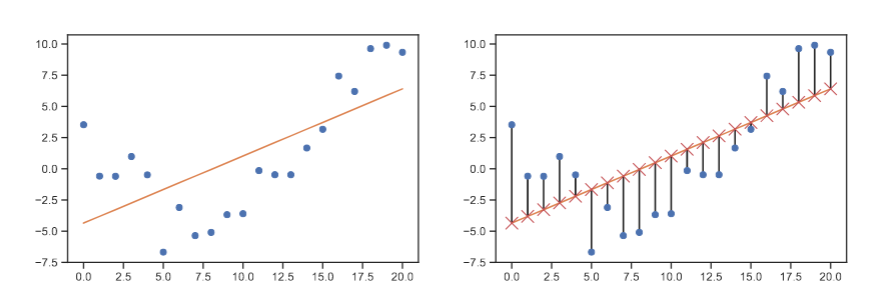
\includegraphics[width=3.5in]{figures/linear_regression.PNG}
    \end{minipage}
    An example of the regression model in 1d data, we can fix the data using the $\textbf{linear regression}$ model.
    \begin{center}
        $f(x;\boldsymbol{\theta})=b+wx$
    \end{center}
    Where w is the $\textbf{slope}$, b is the $\textbf{bias}$, and $\theta$ are the parameters of the model, we can minimize the sum square error.
    \begin{center}
        \[\hat{\boldsymbol{\theta}}=\arg\min_{\boldsymbol{\theta}}MSE(\boldsymbol{\theta})\]
    \end{center}
    If we have multiple input features, we can write
    \begin{center}
        $f(\mathbf{x};\boldsymbol{\theta})=b+w_1x_1+...+w_Dx_D=b+\mathbf{w^Tx}$
    \end{center}
    \begin{minipage}{\linewidth}
            \centering
            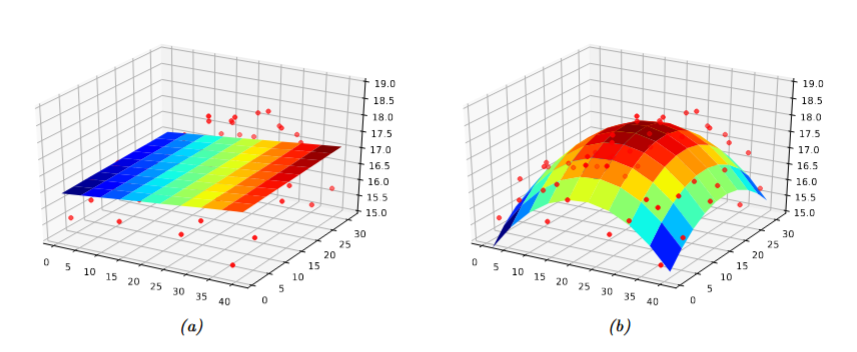
\includegraphics[width=3.5in]{figures/polynomial_regression.PNG}
    \end{minipage}
    We can improve the fit by using a $\textbf{Polynomial regression}$ model with degree $\mathcal{D}$. This now have the form 
    \begin{center}
        $f(x;\mathbf{w})=\mathbf{w^T}\phi(x)$
    \end{center}
    Where $\phi(x)$ are the feature vector derived from the input
    \begin{center}
        $\phi(x)=[1,x,x^2,...,x^D]$
    \end{center}

\subsection{Overfitting}
    Empirical risk (training loss function)
    \[
    \mathcal{L}(\boldsymbol{\theta}; \mathcal{D}_{\text{train}}) = 
    \frac{1}{|\mathcal{D}_{\text{train}}|} 
    \sum_{(\mathbf{x,y}) \in \mathcal{D}_{\text{train}}} 
    \ell(y, f(x; \boldsymbol{\theta}))
    \]

    The difference $\mathcal{L}(\boldsymbol{\theta};p^*)-\mathcal{L}(\boldsymbol{\theta};D_{train})$ called $\textbf{generalization gap}$.
    If a model has a large generalization gap (i.e., low empirical risk but high population risk), it is a sign that it is overfitting. In practice we don't know $p^*$. However, we can partition the data we do have into two subsets, known as the training set and the $\textbf{test set}$. Then we can approximate the population risk using the $\textbf{test risk}$:
    \[
    \mathcal{L}(\boldsymbol{\theta}; \mathcal{D}_{\text{test}}) = 
    \frac{1}{|\mathcal{D}_{\text{test}}|} 
    \sum_{(\mathbf{x,y}) \in \mathcal{D}_{\text{test}}} 
    \ell(y, f(x; \boldsymbol{\theta}))
    \]

    \begin{minipage}{\linewidth}
            \centering
            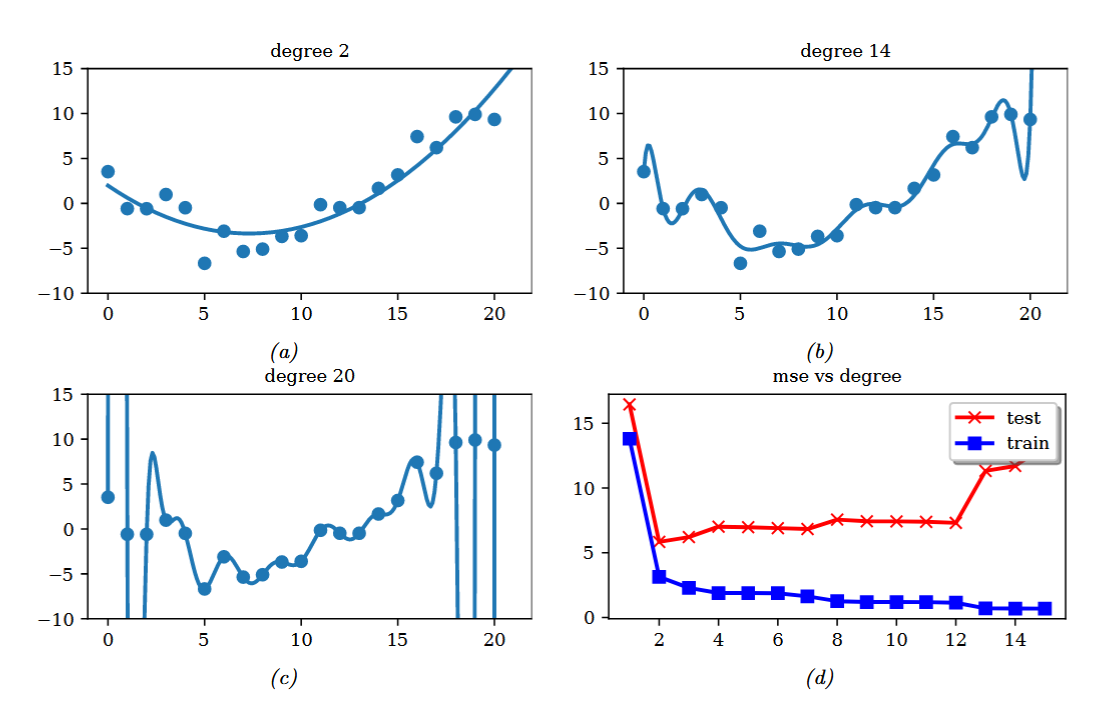
\includegraphics[width=3.5in]{figures/overfitting.PNG}
    \end{minipage}
    
    We can make the training loss function to zero if we increase the degree $\mathcal{D}$, but it will increase the testing loss function. The purpose about the prediction accuarcy on new data, A model that fit the training data but which is too much complex. It will call the $\textbf{overfitting}$. If $\mathbf{D}$ is too small, the model will be $\textbf{underfitting}$.
    
\subsection{Unsupervised learning}
    In supervised learning, we assume that each input $x$ in training set have a output targets $y$, and our goal is to learn the input-output mapping. Although this is useful, and difficult, supervised learning is just a to find a mathematical function to fit the data points. So go back to the unsupervised learning, we will opposed to just learning a mapping. We just get $\mathcal{D} = \{(x_n : n = 1 : N)\}$ without any ouputs $y_n$.This is called $\textbf{unsupervised learning}$.

    From a probabilistic perspective, we can view the task of unsupervised learning as fitting an unconditional model of the form $p(x)$, which can generate new data x, whereas supervised learning involves fitting a conditional model, $p(y|x)$, which specifies (a distribution over) outputs given inputs.

    Unsupervised learning avoids the needs of collect large labeled datasets for training, which can be often time comsuming and expensive and does not rely on manually labeled data or predefined categories, unlike supervised learning, which learns from labeled examples. Instead, unsupervised learning finds patterns, structures, or groupings in the data based on inherent similarities or relationships.
\subsection{Clustering}
    \begin{minipage}{\linewidth}
            \centering
            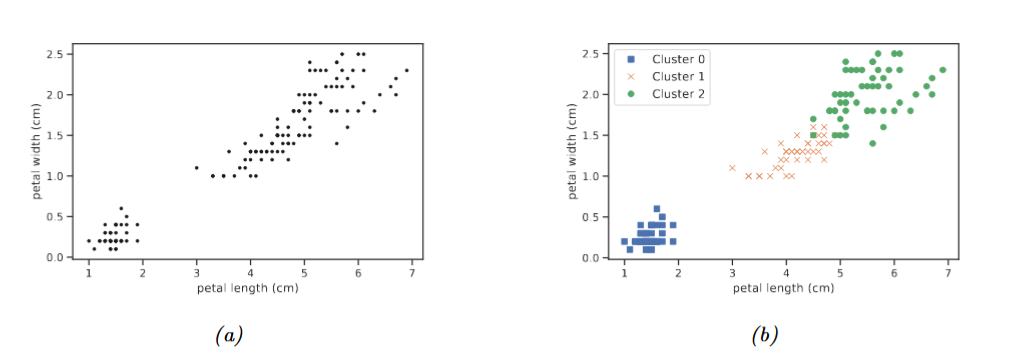
\includegraphics[width=3.5in]{figures/clustering.PNG}
    \end{minipage}
    A simple example of unsupervised learning is the problem of finding clusters in data. The goal is to partition the input into regions that contain “similar” points.
\subsection{Self-supervised learning}
    $\textbf{Self-supervised learning}$ that automatically generating $\textbf{labels}$ from $\textbf{unlabeled data}$. Try to learn to predict a color image from a grayscale image, or to mask out words in a sentence and then try to predict them given the surrounding context. The hope is that the resulting predictor $\hat{x}_1 = f(x_2;\boldsymbol{\theta})$. Where $x_2$ is the observed input and $\hat{x}_1$ is the predict output, will learn useful features from the data, that can be used in standard.
\subsection{Reinforcement learning}
    The system or agent has to learn how to interact with its environment. For example, creating a bot playing Mario, a bot will interact and integration with the world, run left or right or the bot will jump if they see a block stone.(\texttt{\href{https://pytorch.org/tutorials/intermediate/mario_rl_tutorial.html}{Click to see the detail}})
    \begin{minipage}{\linewidth}
            \centering
            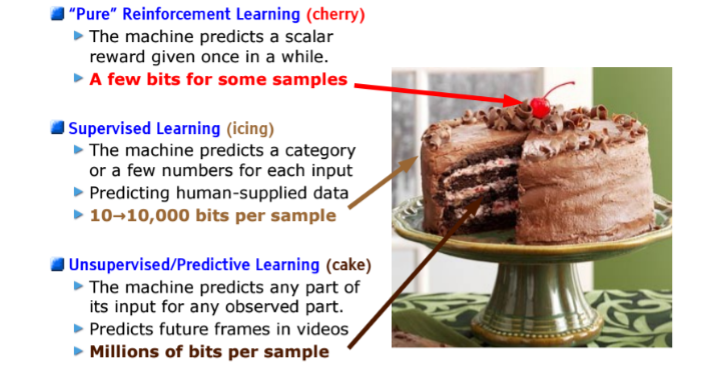
\includegraphics[width=3in]{figures/3typeML.PNG}
    \end{minipage}
\newpage
    
\subsection{Preprocessing discrete input data}
    \textbf{One-hot encoding}

    When we have categorical features, we need to scale it into numerical values, so that the compute makes sense. The standard way to preprocess such categorical variables is to use a $\textbf{one-hot encoding}$. one-hot(x) = $[\mathbb{I}(x=1),...,\mathbb{I}(x=K)]$. If a variable x has $K$ values (3 colors red,green,blue), the corresponding one-hot vectors will be one-hot(red)=[1,0,0], one-hot(green)=[0,1,0], one-hot(blue)=[0,0,1].

    \textbf{Feature crosses}

    Converting the original datasets into a $\textbf{wide format}$, with more many columns. 
    Suppose we want to predict the fuel efficiency of a vehicle given two categorical input variables: 
    \begin{itemize}
        \item \( x_1 \): The type of car (SUV, Truck, Family car).
        \item \( x_2 \): The country of origin (USA, Japan).
    \end{itemize}
    Using one-hot encoding, we represent these variables as separate binary indicators:
    \[
    \phi(x) = [1, I(x_1 = S), I(x_1 = T), I(x_1 = F), I(x_2 = U), I(x_2 = J)]
    \]
    However, this encoding does not capture interactions between the features. For example, we expect trucks to be less fuel-efficient overall, but perhaps trucks from the USA are even less efficient than trucks from Japan. This cannot be captured using a simple linear model.
    We define a new composite feature representing all possible pairs:
    \[
    \text{(Car type, Country)} = \{(S, U), (T, U), (F, U), (S, J), (T, J), (F, J)\}
    \]
    The new model becomes:
    \[
    f(x; w) = w^T \phi(x)
    \]
    Express the equation we have:
    \begin{equation*}
        \begin{split}
            f(x; w) = & \; w_0 + w_1 I(x_1 = S) + w_2 I(x_1 = T) + w_3 I(x_1 = F) \\
            &+ w_4 I(x_2 = U) + w_5 I(x_2 = J) + w_6 I(x_1 = S, x_2 = U) \\
            &+ w_7 I(x_1 = T, x_2 = U) + w_8 I(x_1 = F, x_2 = U) \\
            &+ w_9 I(x_1 = S, x_2 = J) + w_{10} I(x_1 = T, x_2 = J)\\ 
            &+ w_{11} I(x_1 = F, x_2 = J)
        \end{split}
    \end{equation*}

\section{Probability Unvariate Models}\smallskip \hrule height 2pt \smallskip

\subsection{Introduction}
    Calling $\textbf{sample space}$ $\mathcal{X}$ are all possible experiences, and $\textbf{event}$ will be a subset of the $\textbf{sample space}$.
    
    \textbf{Union}
    \[ Pr(A \land B)=Pr(A,B) \]
    If independent events
    \[ Pr(A \land B)=Pr(A)Pr(B) \] 

    We say a set of variables $X_1, . . . , X_n$ is (mutually) independent if the joint can be written as a product of marginals for all subsets $\{X_1,...,X_m\} \subseteq \{X_1,...,X_n\}$
    \begin{equation*}
        p(X_1,X_2,...,X_n)=\prod_{i=1}^{m}p(X_i)
    \end{equation*}
    
    \textbf{Disjoint}
    \[Pr(A \vee B)=Pr(A)+Pr(B)-Pr(A\land B)\]
    \textbf{Conditional probability}
    \[Pr(B|A)\triangleq \frac{Pr(A,B)}{Pr(A)}\]
    If events A and B are conditionally independent given event C
    \[Pr(A,B|C)=Pr(A|C)Pr(B|C)\]
    Be careful, we say $X_1,X_2,X_3$ are mutually independent if the following conditions hold:
    \begin{equation*}
        \begin{split}    
        p(X_1,X_2,X_3)=p(X_1)p(X_2)p(X_3)\\
        ,p(X_1,X_2)=p(X_1)p(X_2) \\
        ,p(X_1,X_3)=p(X_1)p(X_3) \\
        ,p(X_2,X_3)=p(X_2)p(X_3) \\
        \end{split}
    \end{equation*}
    
\subsection{Random variables}
    \begin{minipage}{\linewidth}
            \centering
            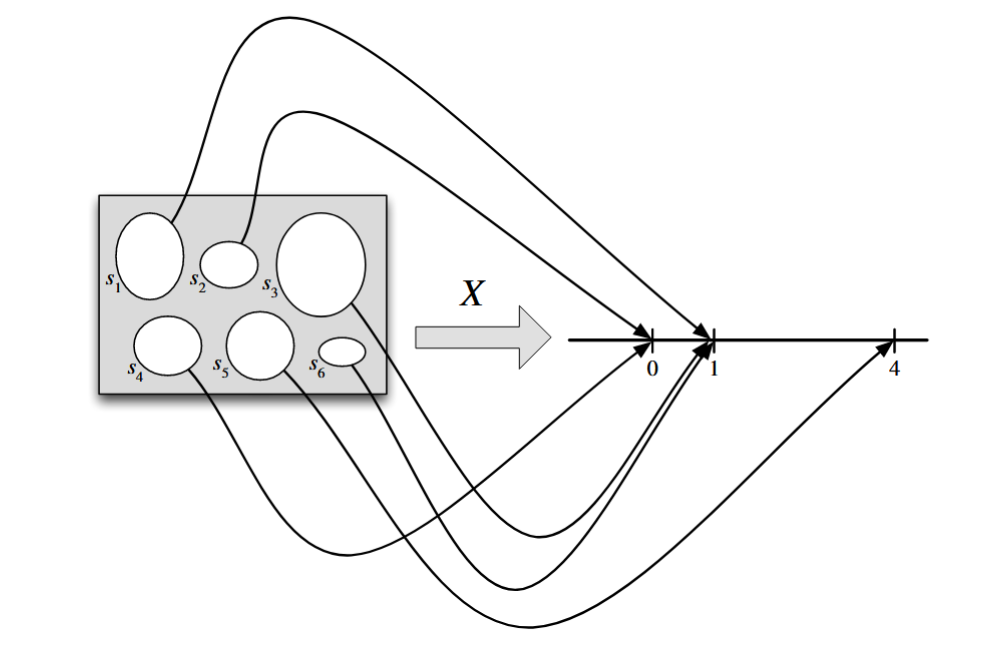
\includegraphics[width=3in]{figures/rv.PNG}
    \end{minipage}
    Given an experiment with sample space $\mathbb{S}$, a random variable(r.v.) is a function mapping from the sample $\mathbb{S}$ to the real value $\mathbb{R}$.
    
    \textbf{Discrete random variables}
    
    If sample space $\mathbb{S}$ have finite or countable, it is called a Discrete r.v. Denote probability of events in $\mathbb{S}$ and have value x by $Pr(X=x)$. This called probability mass function or \textbf{pmf} as a function which compute the probability of events which have the value x.
    \begin{equation*}
        p(x)\triangleq Pr(X=x)
    \end{equation*}
    The pmf satisfied $0\leq p(x) \leq 1$ and $\sum_{x\in \mathcal{X}}^{}p(x)=1$
    
\textbf{Continuous random variables}

    If $X \in \mathbb{R}$, it is called the continuous r.v. The value or no longer create a finite set of distinct possible values it can take on.

\textbf{Cumulative distribution function (cdf)}

    \begin{equation*}
        P(x) \triangleq Pr(X\leq x)
    \end{equation*}

    We can compute the probability of any interval

    \begin{equation*}
        P(a\leq x \leq b) = P(b)-P(a-1)
    \end{equation*}

    In discrete r.v, the cdf will compute
    \begin{equation*}
        P(x)=\sum_{x\in \mathcal{X}}^{}p(x)
    \end{equation*}
    In continuous r.v, the cdf will compute
    \begin{equation*}
        P(x)=\int_{x\in \mathcal{X}}^{}p(x)
    \end{equation*}

\textbf{Probability density function (pdf)}

    Define the pdf as a derivative of the cdf
    \begin{equation*}
        p(x) \triangleq \frac{d}{dx}P(x)
    \end{equation*}
    As the size of interval get smaller, we can write
    \begin{equation*}
        Pr(x<X<x+dx) \approx p(x)dx
    \end{equation*}
    
\textbf{Quantiles}

    If the cdf P is monotonically increase, it has an inverse, called the $\textbf{inverse cdf}$. If P is the cdf of $X$, then $P^{-1}(q)$ is the value $x_q$ that $Pr(X\leq x_q)=q$; this call q'th quantiles of P.    

\textbf{Sets of related random variables}

    Suppose we have two r.v $X$ and $Y$. We can define joint of distribution $p(x,y)=Pr(X=x,Y=y)$ for all possible value of x and y. We can respresent the all possible value by a 2d table. For example:
    \[
    \begin{array}{c|cc}
        p(X,Y) & Y = 0 & Y = 1 \\
        \hline
        X = 0 & 0.2 & 0.3 \\
        X = 1 & 0.3 & 0.2
    \end{array}
    \]
    $Pr(X=0,Y=1)=0.3$, $\sum_{x \in \mathcal{X},y \in \mathcal{Y}}p(x,y)=1$

\textbf{Moments of a distribution}

    $\textbf{Mean}$ is the average of the distribution, other name is called $\textbf{expected value}$, denoted as $\mu$. For continuous r.v, the mean is defined as follow:
    \begin{equation*}
        \mathbb{E}[X]=\int_{x\in \mathcal{X}}xp(x)dx
    \end{equation*}
    If the integral is not finite, the mean is not defined.
    For discrete r.v, the mean is defined as follow:
    \begin{equation*}
        \mathbb{E}[X]=\sum_{x\in \mathcal{X}}xp(x)dx
    \end{equation*}
    Since the mean is linear, we have the \textbf{linearity of expectation}:
    \begin{equation*}
        \mathbb{E}[aX+b]=a\mathbb{E}[X]+b
    \end{equation*}
    For n set random variables, we can show the sum of expectation as follow:
    \begin{equation*}
        \mathbb{E}[\sum X_i]=\sum \mathbb{E}[X_i]
    \end{equation*}
    If they are independent, the expectation of product is defined:
    \begin{equation*}
        \mathbb{E}[\prod X_i]=\prod \mathbb{E}[X_i]
    \end{equation*}
    When we have two or more dependent r.v, we can compute the moment of one given the others. 
    \begin{equation*}
        % \mathbb{E}[X]=\mathbb{E}_Y[\mathbb{E]}]
        \mean[X]=\mean_Y[\mean[X|Y]]
    \end{equation*}
    There is a similar formula for the variance.
    \begin{equation*}
        \var[X]=\mean_Y[\var[X|Y]] +\var_Y[\mean[X|Y]]
    \end{equation*}
    $\textbf{Variance}$ is a measure how "spread" a value compared with the mean of the distribution, denoted as $\sigma^2$. This is define as follow:
    \begin{equation*}
        \begin{split}
        \mathbb{V}[X] \triangleq \mathbb{E}[(X- \mu)^2] =\int(x-\mu)^2p(x)dx \\
        = \int x^2p(x)dx+\mu\int p(x)dx-2\mu\int{xp(x)dx}\\
        =\mathbb{E}[X^2]-\mu^2
        \end{split}
    \end{equation*}
    \begin{minipage}{\linewidth}
            \centering
            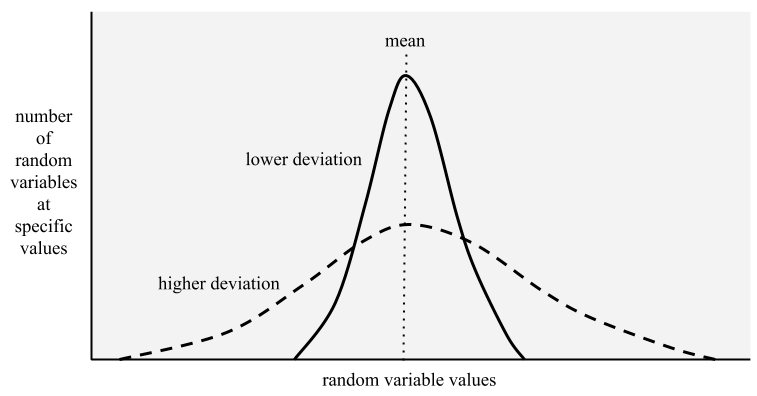
\includegraphics[width=3in]{figures/Variance.png}
    \end{minipage}
    The \textbf{standard deviation} is defined as
    \begin{equation*}
        std[X]=\sqrt{\mathbb{V}[X]}=\sigma
    \end{equation*}
    Lower deviation, the distribution is closer to the mean. High deviation, the distribution is far away from the mean.

    The variance of a shifted and scaled version of a random variable is given by
    \begin{equation*}
        \mathbb{V}[aX+b]=a^2\mathbb{V}[X]
    \end{equation*}

    If we have a set of n independent random variables, the variance of their sum is given by the sum of their variances:
    \begin{equation*}
        \mathbb{V}[\sum X_i]=\sum \mathbb{V}[X_i]
    \end{equation*}
    The variance of their product can also be derived:  
    \begin{equation*}
        \begin{split}
            \mathbb{V}[\prod X_i]= \mathbb{E}[(\prod X_i)^2]-(\mathbb{E}[(\prod X_i)])^2 \\
            = \prod(\sigma_i^2 + \mu_i^2)-\prod\mu_i^2
        \end{split}
    \end{equation*}

    \textbf{Mode of a distribution}
   
    The \textbf{mode} of a distribution is the value with the highest probability mass or probability density
    \begin{equation*}
        \mathbf{x^*}= \arg \max_{\mathbf{x}} p(\mathbf{x})
    \end{equation*}
    If the distribution is multimodal, this may not be unique. Like the function have 2 global extrema(means having 2 highest probability), this can may not be unique.

\subsection{Bayes' Rule}    
\textbf{Bayes' Rule, and with extra conditioning (just add in $C$!)}
         \[P({ A=a}|{ B=b})  = \frac{P({ B=a}|{ A=b})P({ A=a})}{P({ B=b})}\]
         \[P({ A=a}|{ B=b}, { C=c}) = \frac{P({ B=b}|{ A=a}, { C=b})P({ A=a} | { C=c})}{P({ B=b} | { C=c})}\]
  The term \( p(A) \) represents what we know about possible values of \( A \) before we see any data; this is called the \textbf{prior distribution}. (If \( A \) has \( K \) possible values, then \( p(A) \) is a vector of \( K \) probabilities, that sum to 1.) The term \( p(B \mid A = a) \) represents the distribution over the possible outcomes \( B \) we expect to see if \( A = a \); this is called the \textbf{observation distribution}. When we evaluate this at a point corresponding to the actual observations, \( b \), we get the function \( p(B = b \mid A = a) \), which is called the \textbf{likelihood}. (Note that this is a function of \( a \), since \( b \) is fixed, but it is not a probability distribution, since it does not sum to one.) Multiplying the prior distribution \( p(A = a) \) by the likelihood function \( p(B = b \mid A = a) \) for each \( a \) gives the unnormalized joint distribution \( p(A = a, B = b) \). We can convert this into a normalized distribution by dividing by \( p(B = b) \), which is known as the \textbf{marginal likelihood}, since it is computed by marginalizing over the unknown \( A \):

\begin{equation*}
    p(B = b) = \sum_{a' \in \mathcal{A}} p(A = a') p(B = b \mid A = a') 
    = \sum_{a' \in \mathcal{A}} p(A = a', B = b)
\end{equation*}
\textbf{Odds Form of Bayes' Rule}
\[\frac{P({ A}| { B})}{P({ A^c}| { B})} = \frac{P({ B}|{ A})}{P({ B}| { A^c})}\frac{P({ A})}{P({ A^c})}\]
The \emph{posterior odds} of $A$ are the \emph{likelihood ratio} times the \emph{prior odds}. 
\subsection{Bernoulli and binomial distributions}
Given experiment tossing a coin, where the probability of event it lands head is $0\leq\theta \leq 1$, Y = 1 denoted that event, Y=0 denote the events that the coin lands tail. So $p(Y=1)=\theta$ and $p(Y=0)=1-\theta$, This called the $\textbf{Bernoulli distribution}$, it can be written as follows
\[
    Y \sim Ber(\theta)
\]
Where $\sim$ is mean that "is sampled from"
or "is distribution from", Y have model $Ber(\theta)$
The pmf is defined as follow:
\[
    \text{Ber}(y \mid \theta) =
    \begin{cases} 
        1 - \theta & \text{if } y = 0 \\
        \theta & \text{if } y = 1
    \end{cases}
\]
We can also write this:
\[
    \text{Ber}(y \mid \theta) \triangleq \theta^y(1-\theta)^{1-y}
\]
Bernoulli is a special case of $\textbf{Binomial distribution}$. While Bernoulli tossing a coin 1 time, Binomial distribution tossing a coin N times, we observe a set of N Bernoulli trials, denoted $y_n \sim Ber(\cdot\mid\theta)$ (the dot mean that is the placeholder, it can be any specific value (eg. $y=0$ or $y=1$). Define $s$ to be a number of heads, $s \triangleq \sum_{n=1}^{N}\indicator(y_n = 1)$. The distribution of s given by a binomial distribution:
\begin{equation*}
    Bin(s \mid\theta,N) \triangleq \binom{N}{s}\theta^s(1-\theta)^{N-s}
\end{equation*}
When we want to predict a binary variable $y \in \{0, 1\}$ given some inputs $x \in X$ , we need to use a conditional probability distribution of the form
\begin{equation*}
    p(y|\inp,\parameter) = Ber(y\mid f(\inp;\parameter))
\end{equation*}
Where $f(\inp;\parameter)$ is some function that predict the mean parameter of the output distribution. But this will require that $0\leq f(\inp;\parameter)\leq1$ to put into the conditional probability. So to avoid this, we can use any uncontrained function with this:
\begin{equation*}
    p(y|\inp,\parameter) = Ber(y\mid \sigma (f(\inp;\parameter)))
\end{equation*}
Where $\sigma()$ is the \textbf{sigmoid} or \textbf{logistic} function, defined as follows:
\begin{equation*}
    p=logistic(a)=\sigma(a) \triangleq\frac{1}{1+e^{-a}}= \frac{e^x}{1 + e^x}
\end{equation*}
where $a = f(\inp,\parameter)$. The inverse of this is called the $\textbf{logic function}$.
\[
    a=logit(p) =\sigma^{-1}(p) \triangleq \nlogit{p}
\]
So the sigmoid will tranform the function in $\R$ into probability $[0,1]$ and the logit will transform the probability into real numbers, making it easier to model with linear regression techniques.

Some useful properties of these functions.
\[
\sigma(x) \triangleq \frac{1}{1 + e^{-x}} = \frac{e^x}{1 + e^x}
\]

\[
\frac{d}{dx} \sigma(x) = \sigma(x)(1 - \sigma(x))
\]

\[
1 - \sigma(x) = \sigma(-x)
\]

\[
\sigma_+(x) \triangleq \log(1 + e^x) \triangleq \text{softplus}(x)
\]

\[
\frac{d}{dx} \sigma_+(x) = \sigma(x)
\]
\subsection{Categorical and multinomial distributions}
When the Bernoulli have only 2 classes, the categorical will represent a distribution over a finite sets of labels $y \in \{1..C\}$, which generalizes the Bernoulli to $C > 2$ values. The categorical discrete probability distribution with each parameter corresponding to one class.
\[
\text{Cat}(y \mid \parameter) \triangleq \prod_{c=1}^{C} \theta_c^{\mathbb{I}(y=c)}
\]
In other words, $p(y=c \mid\parameter)=\theta_c$. Note that the parameters are constrained so that $0\leq\theta\leq1$. We can write the categorical distribution in another way by converting the discrete variable y into a $\textbf{one-hot vector}$ with C elements. For example, if $C=3$, we encode the classes $1,2$ and $3$ as $(1,0,0),(0,1,0)$ and $(0,0,1)$. 
Consider a fair 6-sided die, where each face corresponds to an outcome:

\[
y \in \{1, 2, 3, 4, 5, 6\}
\]

Each face has an equal probability of occurring, so the categorical distribution parameter \( \theta \) is:

\[
\theta = (\theta_1, \theta_2, \theta_3, \theta_4, \theta_5, \theta_6) = \left( \frac{1}{6}, \frac{1}{6}, \frac{1}{6}, \frac{1}{6}, \frac{1}{6}, \frac{1}{6} \right)
\]

If we roll a 3, then the one-hot encoding for \( y = 3 \) is:
\[
(0, 0, 1, 0, 0, 0)
\]

Substituting into the PMF:

\[
P(y = 3 \mid \theta) = \theta_1^0 \theta_2^0 \theta_3^1 \theta_4^0 \theta_5^0 \theta_6^0
\]

Since any number raised to the power of 0 is **1**, this simplifies to:

\[
P(y = 3 \mid \theta) = \theta_3 = \frac{1}{6}
\]

Thus, for a fair die, the probability of rolling a 3 is \( \frac{1}{6} \).

Using one-hot encoding, each possible outcome can be written as:

\[
\begin{aligned}
y = 1 &\rightarrow (1,0,0,0,0,0) \\
y = 2 &\rightarrow (0,1,0,0,0,0) \\
y = 3 &\rightarrow (0,0,1,0,0,0) \\
y = 4 &\rightarrow (0,0,0,1,0,0) \\
y = 5 &\rightarrow (0,0,0,0,1,0) \\
y = 6 &\rightarrow (0,0,0,0,0,1) \\
\end{aligned}
\]
Now, suppose we have a biased die with the following probabilities:
\[
\theta = (0.10, 0.15, 0.30, 0.20, 0.15, 0.10)
\]

The probability of rolling a 3 is now:

\[
P(y = 3 \mid \theta) = \theta_3 = 0.30
\]
The categorical distribution is a special case of the $\textbf{multinomial distribution}$. Suppose we observe $N$ categorical trials, $y_n \sim Cat(\cdot\mid\parameter)$, for $n = 1 : N$. Think of rolling a C-sided dice $N$ times. Let us define $y$ to be a vector that counts the number of times each face show up
\( y_c = N_c \triangleq \sum_{n=1}^{N} \mathbb{I} (y_n = c) \). Now \( \mathbf{y} \) is no longer one-hot, but is ``multi-hot'', since it has a non-zero entry for every value of \( c \) that was observed across all \( N \) trials. The distribution of \( \mathbf{y} \) is given by the \textbf{multinomial distribution}:

\[
\mathcal{M}(\mathbf{y} \mid N, \parameter) \triangleq 
\binom{N}{y_1 \dots y_C} \prod_{c=1}^{C} \theta_c^{y_c} =
\binom{N}{N_1 \dots N_C} \prod_{c=1}^{C} \theta_c^{N_c}
\]


In the conditional case, we can define

\[
p(y \mid x, \theta) = \text{Cat}(y \mid f(x; \theta))
\]

which we can also write as

\[
p(y \mid x, \theta) = \mathcal{M}(y \mid 1, f(x; \theta))
\]

We require that \( 0 \leq f_c(x; \theta) \leq 1 \) and $
\sum_{c=1}^{C} f_c(x; \theta) = 1.$

To avoid the requirement that $f$ directly predict a probability vector, it common to pass the output from f into the $\textbf{softmax}$ function, also called the $\textbf{multinomial logit}$. It is defined as follows:
\[
    softmax(\mathbf{a})\triangleq
    \begin{bmatrix}
        \frac{e^{a_1}}{\sum_{c'=1}^{C}e^{c'}},...,
        \frac{e^{a_c}}{\sum_{c'=1}^{C}e^{c'}}
    \end{bmatrix}
\]
Similar with sigmoid, it will convert real value $\R^C$ into probability $[0,1]^C$.
But there one weakness in this formula, suppose we have
\[
    p_c=\frac{e^c}{Z(\mathbf{a})}=\frac{e^c}{\sum_{c'=1}^{C}e^{c'}}
\]
Where $\mathbf{a}=f(\inp,\parameter)$, are the logits.
Supose $\mathbf{a}=(1000,1000,1000)$, the computer will compute $inf$. Similarly, $\mathbf{a}=(-1000,-1000,-1000)$ now it will compute $0$. To avoid this, we use the following trick:
\[
    log\sum_{c'=1}^{C}e^{c'} = m +log\sum_{c'=1}^{C}e^{c'-m}
\]
This will hold any $m$, so that the exponential will smaller. It is common to use $m=\max_ca_c$ which ensures the the largest will be zero, so you will definitely not overflow, and even if you underflow, the answer will be sensible. This is known as the $\textbf{log-sum-exp trick}$.
\[
    lse(\mathbf{a})\triangleq \sum_{c'=1}^{C}e^{c'}
\]
Logarithm both side and we have
\[
    p(y=c|\inp)=e^{a_c-lse(\mathbf a)}
\]

\end{multicols*}

\end{document}